\documentclass[10pt,a4paper]{article}
\usepackage{fontspec,polyglossia}\setmainlanguage{russian}\setmainfont{Times New Roman}
\usepackage{amsmath,amssymb,booktabs,tabularx,graphicx}\usepackage[margin=17mm]{geometry}
\usepackage[hidelinks]{hyperref}\usepackage{titlesec}\titleformat{\section}{\large\bfseries}{}{0pt}{}
\titlespacing*{\section}{0pt}{8pt}{4pt}\setlength{\parindent}{0pt}\setlength{\parskip}{4pt}\setlength{\emergencystretch}{3em}
\begin{document}
{\Large\bfseries Walker2d: как MG реагирует на силу сглаживания политики}\par\medskip

\section*{Главный результат}

На пяти новых сидах умеренное сглаживание обучаемой политики уменьшает MG нормы управляющего действия: на 20\% при $\lambda=0.25$ и на 40\% при $\lambda=1$ (медианы парных отношений). Знак воспроизводится на всех пяти сидах и трёх агрегированных управляющих логах. При чрезмерном штрафе $\lambda=4$ команды ещё плавнее, но агент часто падает, а MG нормы действия обычно растёт. Это подтверждает чувствительность MG к изменению структуры управляющего лога, но не доказывает уменьшение размерности всей системы или выигрыш по времени.

\section*{Кто учится, чему и зачем}

Агент Walker2d получает 17 наблюдений о положении и скорости тела и выдаёт шесть управляющих команд суставам. PPO дообучает уже ходящую политику из одного общего сохранённого состояния. Актор и критик имеют отдельные сети 64--64 с Tanh. Практический мотив постановки: уменьшить резкость команд, сохранив ходьбу и исходную награду среды. Энергопотребление, износ и перенос на реального робота здесь не измерялись.

К стандартной функции потерь PPO добавлен штраф

\[
L=L_{\mathrm{PPO}}+\lambda\,\mathbb{E}_{(s_t,s_{t+1})}\frac{1}{6}\|\bar a_\theta(s_{t+1})-\bar a_\theta(s_t)\|_2^2,
\qquad \bar a_\theta(s)=\operatorname{clip}(\mu_\theta(s),-1,1).
\]

Здесь $\mu_\theta$ --- среднее распределения действий политики; пары состояний берутся из текущего rollout без переходов между эпизодами. На каждом минибатче берётся столько случайных пар, сколько в нём действий. Штраф действует на средние команды, а не на шум исследования; награда среды не меняется. Измеряем динамику действий и движения при фиксированной политике каждого чекпоинта, затем сравниваем эти диагностики между этапами обучения. Это не MG по последовательности весов сети или training loss.

\section*{План и точные параметры}

Пилот: сид 230, четыре значения $\lambda\in\{0,0.25,1,4\}$, пять reset 61001--61005. Сохранены проверки трёх поздних чекпоинтов; решение продолжить принято по финальному, без MG: умеренные штрафы сохранили ходьбу и награду. Подтверждение: все четыре коэффициента, пять новых сидов 231--235, десять одинаковых тестовых reset 62001--62010. Итого 20 новых обучений и 200 финальных тестов; пилот в итоговые числа не включён. Тестовые reset уже использовались в предыдущих опытах этой серии, поэтому это новые обучающие сиды, но не полностью новый набор начальных состояний.

Каждое обучение: 1048576 дополнительных переходов, 8 сред, rollout 512 шагов на среду, batch 256, 5 эпох PPO, learning rate от $3\cdot10^{-5}$ до $3\cdot10^{-6}$, clip 0.1, target KL 0.01, $\gamma=0.99$, GAE 0.95, entropy coefficient 0, value coefficient 0.5, gradient clipping 0.5. Статистика нормализации наблюдений и наград заморожена из общего anchor. Среда обучения ограничена 5000 шагами на эпизод.

Тест: детерминированная политика, 512 шагов разогрева, затем 4096 шагов записи, шаг времени 0.008 с. Успех: полная запись без падения и средняя скорость не меньше 0.5. Допуск к анализу требует также стандартного отклонения правого колена не меньше 0.05 и как минимум восьми пиков (расстояние 20, prominence 0.15). Награда усредняется на фиксированных 4096 шагах; после падения остаток получает нулевой вклад. Поэтому короткий эпизод не выглядит успешным.

\section*{Что измеряется}

$a_t\in\mathbb{R}^6$ --- исполненная команда. Независимые от MG показатели плавности:

\[
J_1=\frac{\sum_{t=1}^{T-1}\|a_t-a_{t-1}\|_2^2}{6(T-1)},\qquad
J_2=\frac{\sum_{t=2}^{T-1}\|a_t-2a_{t-1}+a_{t-2}\|_2^2}{6(T-2)},\qquad T=4096.
\]

$J_1$ близок к обучающему штрафу; $J_2$ проверяет вторые разности. Снижение обоих означает более плавные команды, но само по себе не устанавливает уменьшение числа степеней свободы. Их абсолютные значения чувствительны к масштабу действий.

\newpage

Для проверки всего движения используем $x_t=(q_{t,1:},\dot q_t/5)\in\mathbb{R}^{17}$: горизонтальная координата переноса исключена, остальные восемь координат положения и девять скоростей сохранены. Определим $V=T^{-1}\sum_t\|x_t-\bar x\|_2^2$. Тогда

\[
R=\min_{p\in\{20,\ldots,250\}}\frac{\frac{1}{T-p}\sum_{t=0}^{T-p-1}\|x_{t+p}-x_t\|_2^2}{2V},\qquad
D=\frac{\frac{1}{K}\sum_{i=1}^{K}\|z_i-\bar z\|_2^2}{V}.
\]

$R$ --- ошибка повторения полного состояния через общий лаг; $D$ --- разброс $K$ состояний $z_i$ около максимумов угла правого колена. Время пика уточняется параболой по трём точкам, состояние --- линейной интерполяцией. Меньшие значения означают лучшую повторяемость по соответствующему критерию. Ни одна из величин не является точной размерностью; повторяемость во времени и повторяемость в выбранной фазе могут расходиться.

Основной скаляр для MG: $\|a_t\|_2$. Дополнительные: $\|a_t-a_{t-1}\|_2$ и среднее шести команд. Настройки перенесены из предыдущего опыта: окно 2048, задержка 8, вложение $E=20$, 20 соседей, исключение Theiler 312, dither $10^{-9}$, seed оценщика 123; дополнительно сохранён результат $E=40$. По траектории берётся медиана трёх окон с концами 2048, 3072, 4096. Для допуска требуем отсутствие численного вырождения во всех трёх окнах. Все 169 допущенных финальных траекторий прошли эту проверку; она не равнозначна подтверждению всех теоретических предпосылок.

\section*{Финальные результаты: все пять новых сидов}

Ниже диагностики --- отношения к $\lambda=0$: сначала медиана по общим допустимым reset внутри сида, затем медиана по пяти сидам. Эти пять сидов --- повторения обучения; 50 эпизодов не считаются 50 независимыми обучениями. Успех и награда учитывают все эпизоды, включая падения. Награда в таблице --- отношение средних по всем 50 эпизодам, а не медиана отношений по сидам.

\begin{center}\small
\begin{tabularx}{\linewidth}{l>{\raggedright\arraybackslash}X>{\raggedright\arraybackslash}X>{\raggedright\arraybackslash}X>{\raggedright\arraybackslash}X>{\raggedright\arraybackslash}X>{\raggedright\arraybackslash}X>{\raggedright\arraybackslash}X>{\raggedright\arraybackslash}X}
\toprule
$\lambda$ & Успех & Общих пар & Награда & MG нормы & $J_1$ & $J_2$ & $R$ & $D$ \\
\midrule
0 & 48/50 & 48 & 1.000 & 1.000 & 1.000 & 1.000 & 1.000 & 1.000 \\
0.25 & 49/50 & 47 & 1.020 & 0.801 & 0.539 & 0.385 & 0.650 & 1.281 \\
1 & 47/50 & 45 & 0.978 & 0.604 & 0.331 & 0.181 & 0.508 & 1.157 \\
4 & 25/50 & 24 & 0.681 & 1.114 & 0.180 & 0.064 & 2.029 & 0.971 \\
\bottomrule\end{tabularx}\end{center}

\begin{center}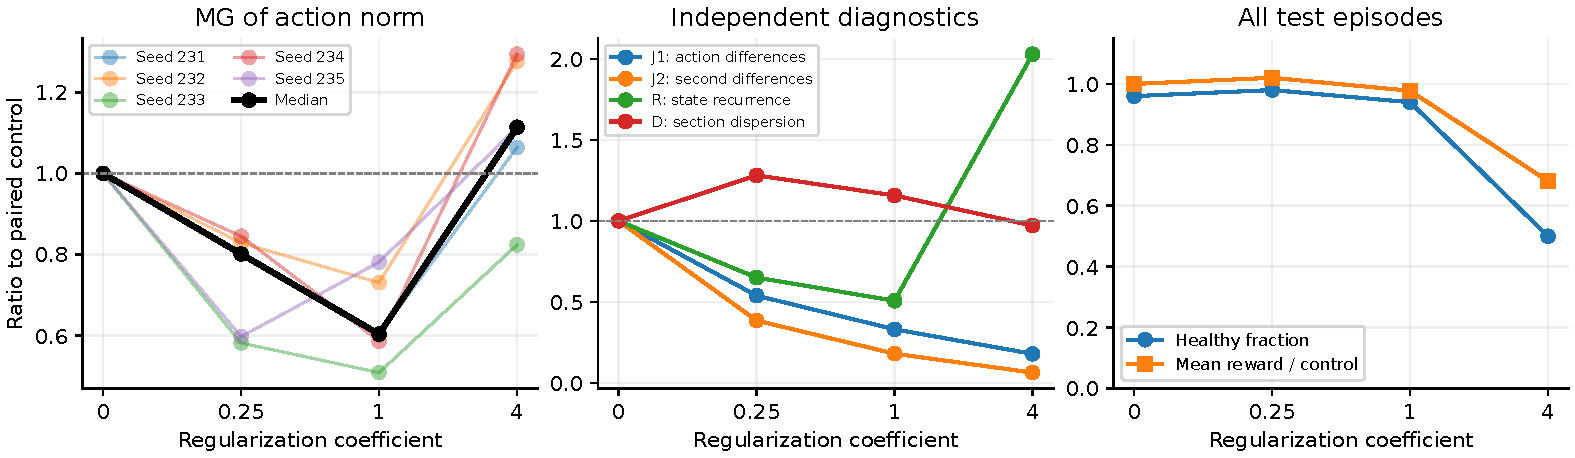
\includegraphics[width=\linewidth,height=.32\textheight,keepaspectratio]{lambda_comparison.pdf}\end{center}

Для $\lambda=0.25$ отношения MG нормы по отдельным сидам лежат в диапазоне 0.582--0.845; для $\lambda=1$ --- 0.509--0.781. Все пять уменьшаются. Дополнительные скаляры подтверждают знак: MG нормы приращения равен 0.662 и 0.601; MG среднего действия --- 0.742 и 0.651 соответственно. Коэффициенты и основной скаляр не выбирались по этим результатам. Полностью монотонного эффекта по силе штрафа нет: на сиде 235 MG при $\lambda=1$ выше, чем при 0.25.

$R$ уменьшается на 4/5 сидов при $\lambda=0.25$ и 5/5 при $\lambda=1$, но $D$ растёт на 5/5 и 4/5 соответственно. Значит, независимое подтверждение относится прежде всего к плавности команд и одному критерию повторяемости, а не ко всем аспектам динамики. При $\lambda=4$ MG нормы растёт на 4/5 сидов при ухудшении ходьбы. Это различает сглаживание и деградацию в данном опыте, но не является проверенным универсальным детектором отказов. В этой группе анализ выживших особенно смещён: на сиде 232 осталась только одна общая пригодная пара.

\newpage

\section*{Что происходит по ходу обучения}

Дополнительно проверены пять фиксированных чекпоинтов всех 20 политик на одном заранее выбранном reset 62001. Настройки MG и трёх окон те же. Упавшие эпизоды не получают нулевой MG: пары исключены из медианы данного этапа, их число указано в скобках.

\begin{center}\small
\begin{tabularx}{\linewidth}{l>{\raggedright\arraybackslash}X>{\raggedright\arraybackslash}X>{\raggedright\arraybackslash}X}
\toprule
Переходы & MG, $\lambda=0.25$ & MG, $\lambda=1$ & MG, $\lambda=4$ \\
\midrule
0 & 1.000 (5) & 1.000 (5) & 1.000 (5) \\
262144 & 0.811 (5) & 0.749 (3) & 0.796 (4) \\
524288 & 0.808 (5) & 0.838 (4) & 0.731 (2) \\
786432 & 0.747 (4) & 0.827 (5) & 1.022 (3) \\
1048576 & 0.745 (5) & 0.531 (4) & 1.052 (3) \\
\bottomrule\end{tabularx}\end{center}

\begin{center}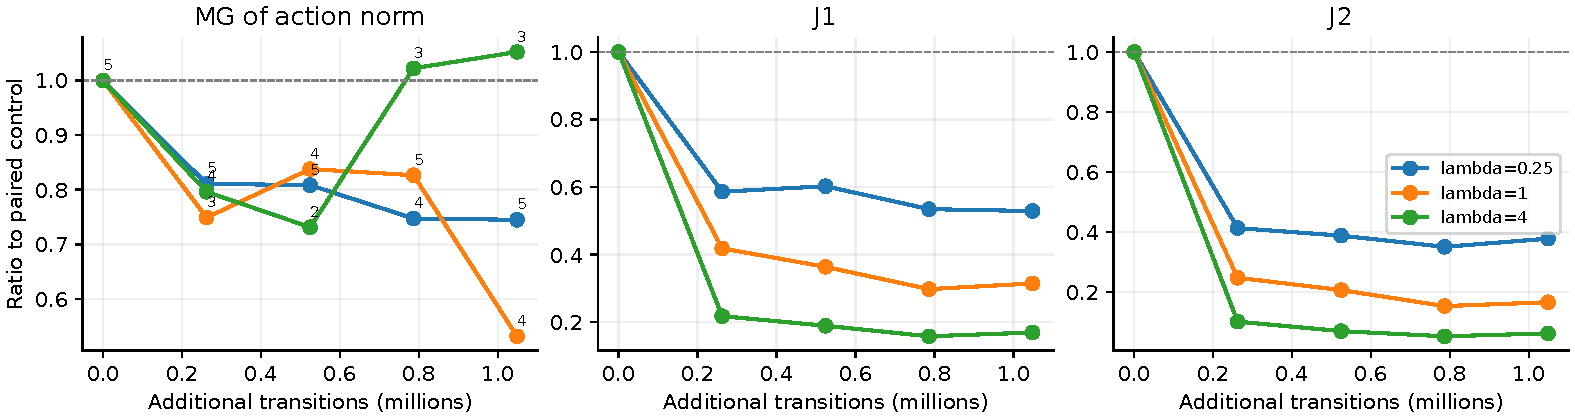
\includegraphics[width=\linewidth,height=.32\textheight,keepaspectratio]{lambda_timecourse.pdf}\end{center}

При умеренных штрафах уменьшение MG появляется уже после первого проверенного этапа обучения. При сильном штрафе к концу MG возвращается к контролю или превышает его, хотя $J_1/J_2$ остаются низкими. Из-за изменения состава выживших пар эти медианные кривые нельзя трактовать как непрерывную траекторию одной системы; данные каждого сида сохранены отдельно.

\section*{Вычислительная стоимость}

Последовательный CPU-замер на одной сохранённой траектории контроля (сид 231, reset 62001), один численный поток, прогрев и пять повторов, медиана. Чтение файла, симуляция и подготовка скалярного лога не включены. Сравнение $R,D$ доступно как на 2048, так и на 4096 точках; размер состояния здесь всего 17.

\begin{center}\small
\begin{tabularx}{\linewidth}{l>{\raggedright\arraybackslash}X}
\toprule
Диагностика & Время, с \\
\midrule
$J_1$ и $J_2$, 4096 точек & 0.000124 \\
$R$ и $D$, 2048 точек полного состояния & 0.0266 \\
$R$ и $D$, 4096 точек полного состояния & 0.0523 \\
MG, одно окно 2048, $E=20$ & 0.455 \\
MG плюс проверка $E=40$, одно окно & 0.941 \\
MG плюс проверка $E=40$, три окна & 2.910 \\
\bottomrule\end{tabularx}\end{center}

В этой реализации MG примерно в 17 раз медленнее $R,D$ на одинаковом числе точек. Он требует один скаляр вместо полного состояния, но уменьшение требований к наблюдениям не означает выигрыш по времени. $J_1/J_2$ существенно дешевле, если задача --- только контроль плавности. Преимущество MG по сравнению со спектрами Ляпунова или высокоразмерными эталонами этот опыт не проверяет.

\section*{Вывод для статьи и границы результата}

Корректный тезис: при дообучении управляющей политики с умеренной временной регуляризацией MG по одному агрегированному логу устойчиво обнаруживает изменение, сопровождаемое снижением резкости команд и ошибки повторения состояния; эффект подтверждён на пяти новых сидах. При чрезмерной регуляризации связь нарушается, что видно при совместном контроле качества и диагностик.

Вмешательство прямо поощряет гладкость, все политики происходят из одного anchor, а $D$ не подтверждает общего упрощения движения. Отношение MG при $E=40$ и $E=20$ не всегда близко к единице. Поэтому точное число компонент, причинная связь MG с качеством и преимущество по скорости не установлены. Для усиления нужны независимо обученные anchor и изменение структуры, не заданное штрафом.

Данные по сидам и команды воспроизведения перечислены в README.md. Отчёт: 30 сентября 2026 года; основная статья не менялась.
\end{document}